\subsection{Overview}
CLup's architecture is layered as follows:
\begin{itemize}
	\item \textbf{Presentation layer} (P) handles the interaction with users. It contains the interfaces able to communicate with them and it is responsible for rendering of the information. Its scope is to make understandable the functions of the application to the customers.
	\item \textbf{Application layer} (A) takes care of the functions to be provided for the users. It also coordinates the work of the application, making logical decisions and moving data between	the other two layers.
	\item \textbf{Data access layer }(D) which takes care of the information management, database access control. It also handles data retrieval and passes them to upper level layers.
\end{itemize}
 
The architecture style chosen for CLup is the \textbf{multi-tier} one.
As previously anticipated in the Requirements Analysis and Specifications Document, there will be at least one server for each one of the following interest areas:
\begin{itemize}
    \item Bookings
    \item Queues
    \item Notifications
    \item Stores
    \item Staff members
    \item Customers
\end{itemize}

This is mainly done to distribute workload as well as making the overall system more robust.

There will be also at least two servers for the two following functionalities:
\begin{itemize}
    \item Customer related functionalities
    \item Staff related functionalities
\end{itemize}
The bookings, queue and notifications databases will be distributed and replicated all over the entire store list. Each store will have its own instance of bookings, queue and notifications database while a central logic server will act as a request redirector towards them whenever needed.\\

In Figure \ref{fig:HLArch} is represented the high-level architecture of the system: customers clients, through an internet connection, can connect to Clup's Web Servers.Client's operations are redirected by Web Servers to the Central Customer Operations Manager, who represents the A layer of the customers' side, and, depending by the kind of information, stored or retrieved on the Customers Database or in one of the three local store databases: Bookings, Notifications, Queue. Staff clients instead are connected through a LAN connection to their Local Web Server, who will redirect their requests to the Staff Operations Manager server. This machine is expected to process the logic of requests and then submit them to the Local Application Logic server who will decide in which database store or retrieve the information. Local Application Servers are connected to the Central Customer Operations Manager as well through an internet connection.
\begin{figure}[h!]
	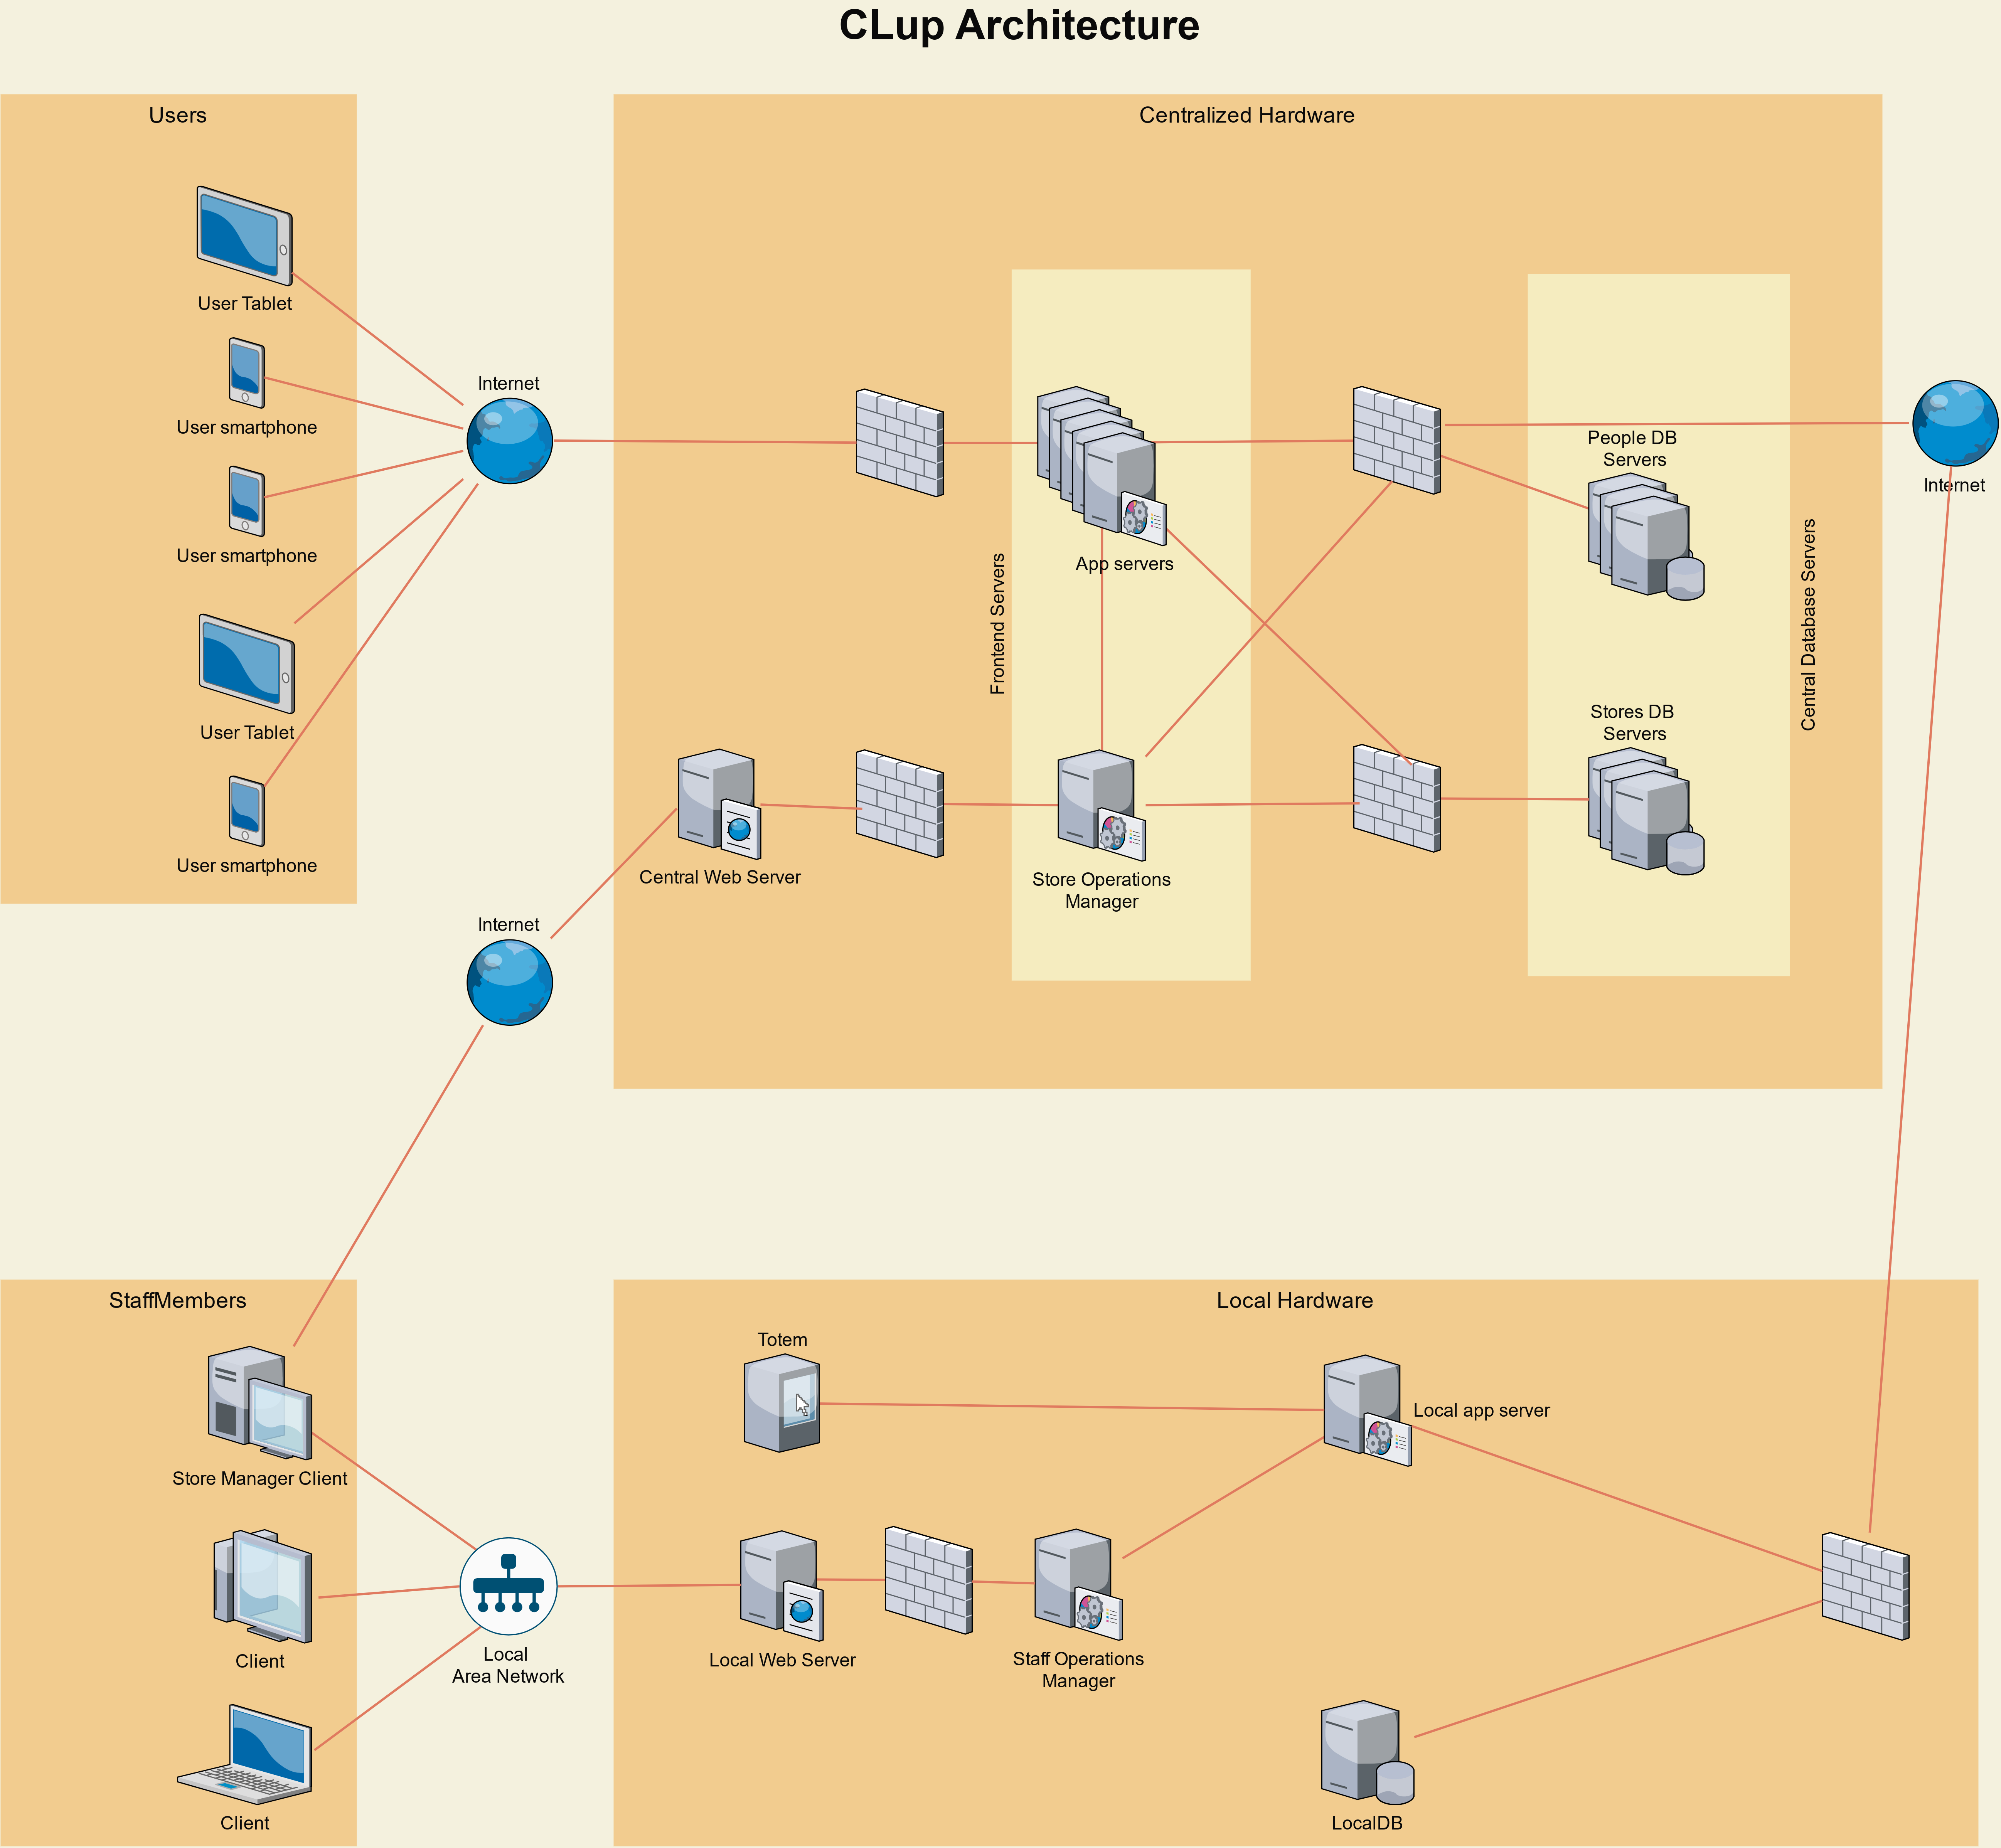
\includegraphics[width=\linewidth]{../Diagrams/Archtecture/Architecture_diagram.png}
	\caption{High-level architecture}
	\label{fig:HLArch}
\end{figure}

\subsection{Component view}
%Worst screenshot ever
\begin{figure}[h!]
	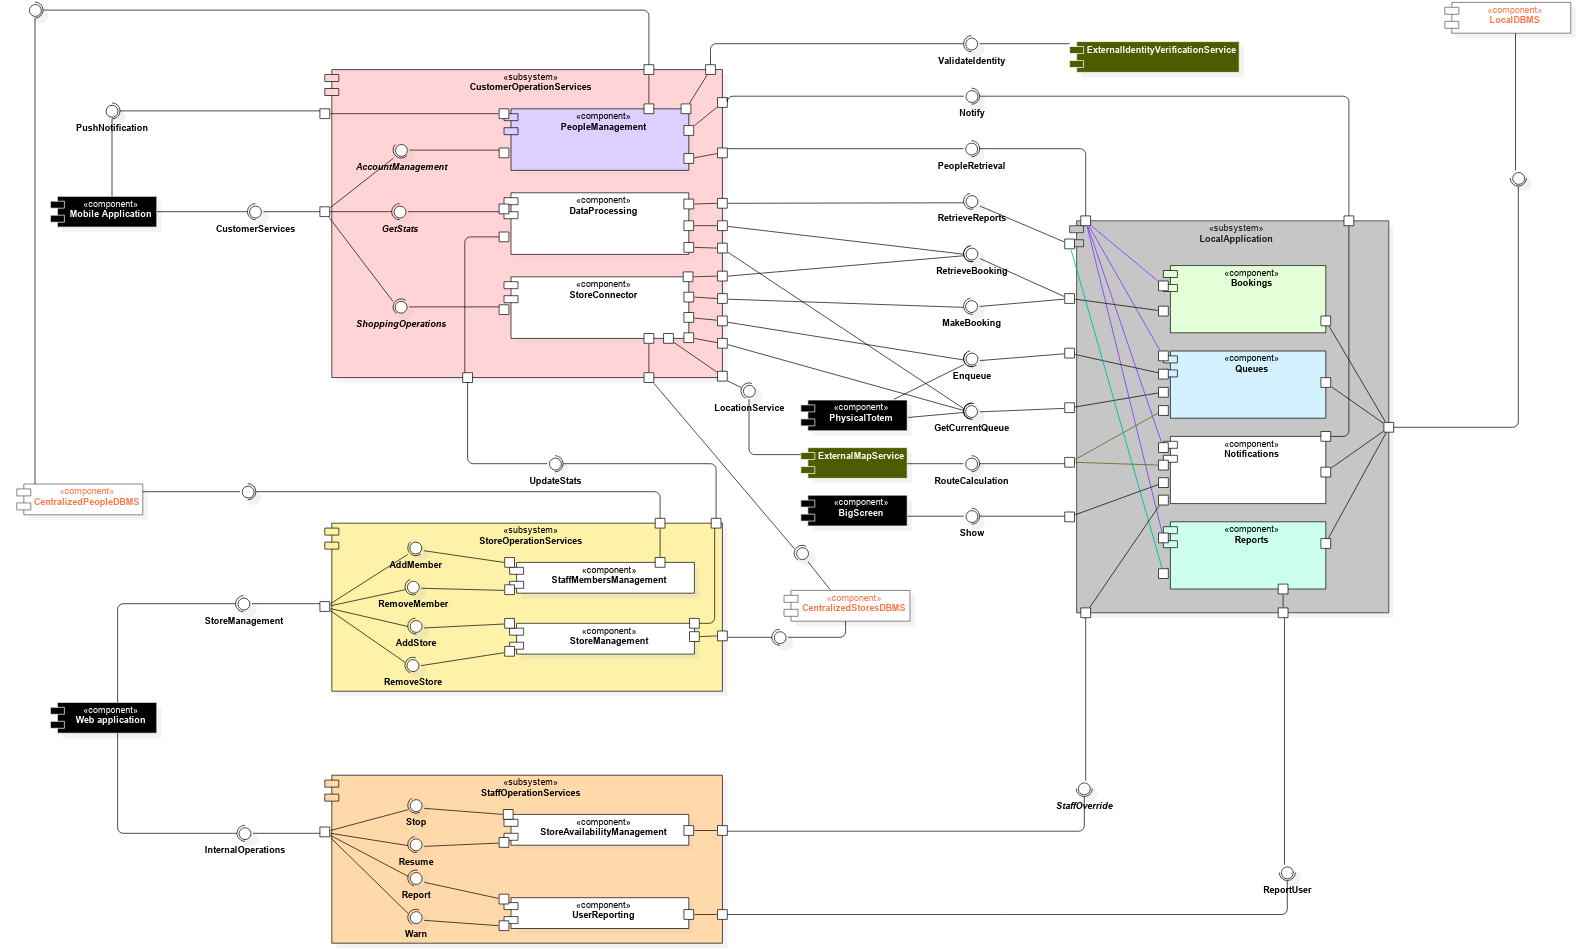
\includegraphics[width=\linewidth]{../Diagrams/ComponentDiagram.png}
	\caption{Component Diagram}
	\label{fig:CompDgm}
\end{figure}
In Figure \ref{fig:CompDgm} is represented the component diagram of the
internal structure of the application server \textbf{TODO: ci sono diversi A server, di conseguenza bisognerebbe dividere il component diagram}, showing how its components interact. The application server
contains Clup's business logic. What follows is a brief description of every component:
\begin{itemize}
	\item \textbf{Staff Web Services}: this component is made of two subcomponents that provide logic and interface to the web application used by store managers:
	\begin{itemize}
		\item \textbf{Store Manager}: This component is responsible for the subscription and the unsubscription 
		\item \textbf{Store Activity Manager}:This component provides the information about people fluxes and the functionalities provided to store managers
	\end{itemize}
	\item \textbf{Customer Services}: This component has a subcomponent \textbf{Service Redirector} that, depending on the the customer's request, forwards it to the right interface
	\item \textbf{Queue Services}: This component aims at managing and updating supermarket's lines 
	\item \textbf{Bookings Services}: This is the component who manages customer's bookings and store's calendar and slots 
	\item \textbf{User Services}:This component has two subcomponents:
	\begin{itemize}
		\item \textbf{Customers}: Here the logic of Clup handles customer information 
		\item \textbf{Staff}: Here Clup's logic handles Staff information
	\end{itemize}
	\item \textbf{Application Logic TODO: change this name}:
	\item \textbf{External Map Services}: This is the component that provides the map interface
\end{itemize}
Nearly every component interacts with the database system to store or retrieve the information.
\subsection{Deployment view}
\subsection{Runtime view}
\subsection{Component interfaces}
\subsection{Selected architectural styles and patterns}
\subsection{Other design decisions}
